\documentclass[10pt]{sig-alternate}
\makeatletter
\def\@copyrightspace{\relax}
\makeatother

\usepackage{hyperref}
\usepackage{listings}

\newcommand{\quotes}[1]{``{#1}''}

\usepackage{xcolor}

\colorlet{punct}{red!60!black}
\definecolor{background}{HTML}{EEEEEE}
\definecolor{delim}{RGB}{20,105,176}
\colorlet{numb}{magenta!60!black}

% There is no lst-language highlighting json code nicely. Hence, we define it here.
\lstdefinelanguage{json}{
    basicstyle=\normalfont\ttfamily,
    numbers=left,
    numberstyle=\scriptsize,
    stepnumber=1,
    numbersep=8pt,
    showstringspaces=false,
    breaklines=true,
    frame=lines,
    backgroundcolor=\color{background},
    literate=
     *{0}{{{\color{numb}0}}}{1}
      {1}{{{\color{numb}1}}}{1}
      {2}{{{\color{numb}2}}}{1}
      {3}{{{\color{numb}3}}}{1}
      {4}{{{\color{numb}4}}}{1}
      {5}{{{\color{numb}5}}}{1}
      {6}{{{\color{numb}6}}}{1}
      {7}{{{\color{numb}7}}}{1}
      {8}{{{\color{numb}8}}}{1}
      {9}{{{\color{numb}9}}}{1}
      {:}{{{\color{punct}{:}}}}{1}
      {,}{{{\color{punct}{,}}}}{1}
      {\{}{{{\color{delim}{\{}}}}{1}
      {\}}{{{\color{delim}{\}}}}}{1}
      {[}{{{\color{delim}{[}}}}{1}
      {]}{{{\color{delim}{]}}}}{1},
}



\begin{document}

% Copyright
\setcopyright{acmcopyright}

\title{
  % 
\includegraphics[width=0.2\textwidth]{hpi_logo_2017}\\
  \vspace{24pt}
  % In-Memory Trajectory Analysis on Taxi Data
  Comparison of Different Data Layouts for Columnar In-Memory Databases on the Basis of an Example Application
}
\subtitle{
  Seminar Trends and Concepts 3\\
  Summer Semester 2018
}

\numberofauthors{3}

\author{
  Marcel Jankrift, Sebastian Kliem, Toni Stachewicz\\[12pt]
  Supervisors:\\
  Dr. Matthias Uflacker, Keven Richly
}


\maketitle
\begin{abstract}
With a strongly increasing number of GPS equipped devices that generate trajectory information, analyzing and using this data catches more and more attention. That is why besides using some specialized trajectory processing systems for that kind of data the interest in using common databases for this task rises. This is the case especially for columnar in-memmory systems. We compare three different data layouts which are designed such databases based on a real-world usecase. Therefore we developed an example application with taxi data and benchmarked those data layouts against typical queries of our usecase.
\end{abstract}

% looks awkward without line break
\keywords{Geospatial data, Trajectory analysis, Taxi data,\\In-Memory}

\section{Motivation}

Storing trajectory data in traditional relational da\-ta\-ba\-ses is not always the best idea. Requests might take a long time when working on big datasets. It is also difficult to achieve good compression rates. There exist some systems which are purely designed to work with such trajectories. Those systems are performing much better than the traditional databases.

In our project investigated how a columnar in-memory database can handle trajectory data. Thereby, we can make use of the in-memory architecture and the columnar storage benefits. We developed an example application which covers a lot of real world requests to a large trajectory dataset. This application builds a good basis to benchmark different data layouts and optimizations.

Traditional taxi companies like to increase their profit. For that, the individual taxi drivers would have to find many passengers and minimize their waiting times. A way to be a good performing taxi is to stay in a profitable area of the city. For example, where taxi rides are highly needed at a specific time. With our help, the taxi companies can develop new strategies. A simple strategy would be to only accept and assign orders whose destination is in a good area for the expected arrival time. We created an interactive map, which shows the best performing taxis for one day in Shenzhen. This is based on a dataset that is explained in section \ref{sec:ds}. The application has some additional information about the taxi density and numbers about pick-ups and drop-offs. Taxi companies could use the application to quickly analyze the collected GPS data.

\section{Data Sources}
\label{sec:ds}

The data we used is a freely available collection of GPS information of taxis.\footnote{\href{https://www-users.cs.umn.edu/~tianhe/BIGDATA/UrbanCPS/TaxiData/TaxiData}{https://www-users.cs.umn.edu/$\sim$tianhe/BIGDATA/\\UrbanCPS/TaxiData/TaxiData}} The dataset has been collected over one day starting at 12~AM and ending at 23:59~PM in the city of Shenzhen, China and the surrounding area. The data does not only contain the GPS location at a certain time, but also the current speed and the taxi's occupancy. The status of a driving taxi has been recorded in an average interval of 26.85 seconds or every 15 seconds in median. In total there are 14,728 trajectories traced resulting in almost 47 million records. The data comes in CSV-format which can be loaded into the SAP HANA database immediately. One sample point contains six attributes: trajectory id (TID), longitude, latitude, timestamp, speed and a flag indicating the presence of a passenger.

\subsection{Data Cleansing}
Before we started analyzing the trajectories we had a closer look at the dataset itself. We noticed rather soon, that there are some inconsistencies within the data. Hence, we perform data cleansing. In the following paragraphs, we describe our criteria for data cleansing in detail.

\subsubsection{Duplicates}
The data was already imported into the database by our supervisor, when we started our project. Since we did not want to change the original data, we created an own table. Once we wanted to create a primary key on it, the database has thrown an error stating that the data has duplicate values. In fact, there are 381 data points occuring not only twice, but also multiple times. We deleted those entries, because they do not add any value to the data and prevent the creation of a primary key.

\subsubsection{Bounding box}
Generally, GPS coordinates are not completely accurate. However, there are points in the dataset, that do not make sense, are not even possible or do not fit into the geospatial system of longitudes and latitudes. The graphic \ref{fig:bbox} below shows the trajectory with id \textit{22,360} which passes through the ocean. In order to eliminate such outliers, we use a bounding box (rectangle highlighted in red color). To avoid deleting points that are outside this area, because a taxi really drove there, we have chosen the rectangle intentionally large. This data cleansing step effects almost 8,000 GPS points.

\begin{figure}[ht]
\centering
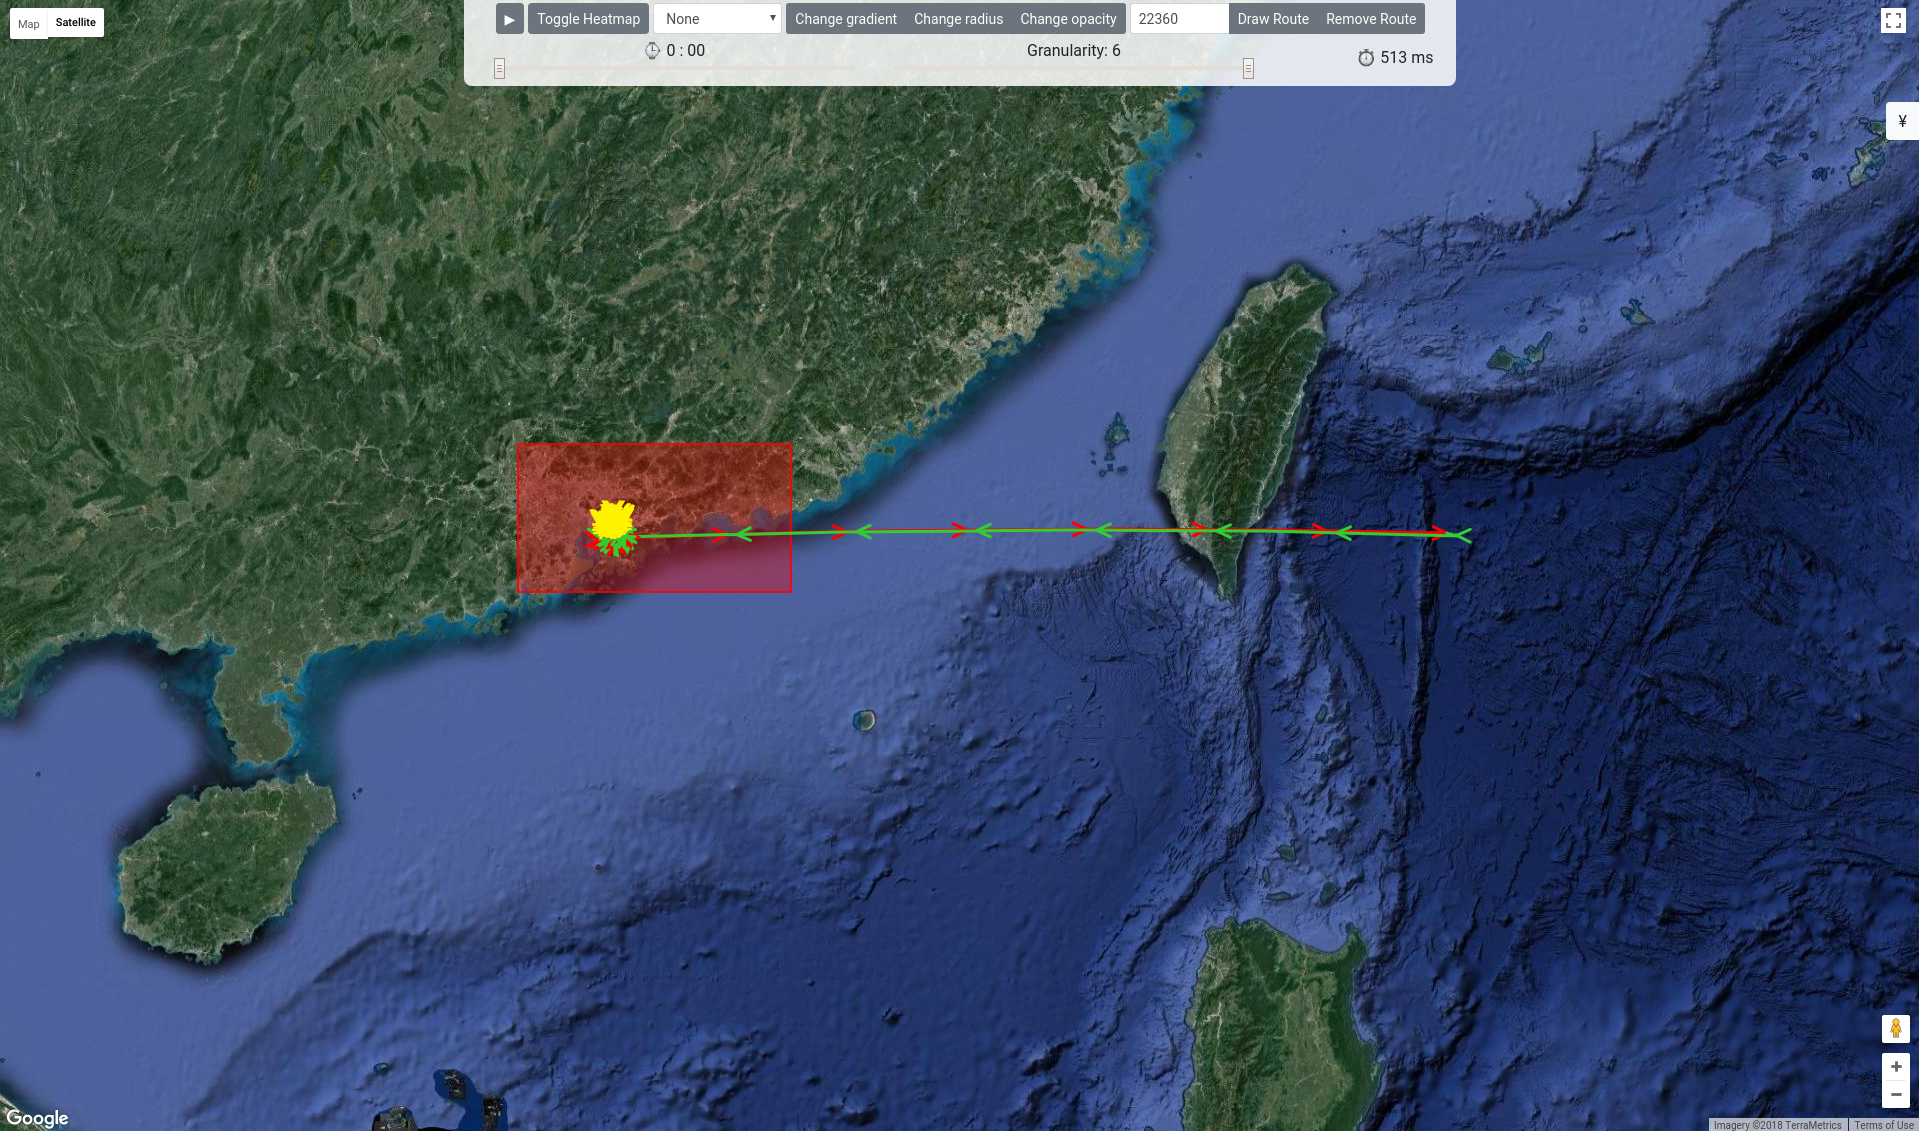
\includegraphics[width=0.5\textwidth]{img/bounding_box.png}
\caption{Bounding box and trajectory \textit{22,360} passing through the ocean}
\label{fig:bbox}
\end{figure}


\subsubsection{Small trajectories}
Some trajectories have only a few data points. The reasons for that can be of different nature. Some trajectories include only a few minutes instead of a whole day. Others have breaks lasting a couple of hours. We also noticed, that some taxis have a different time interval in terms of sending GPS locations, for example only every five minutes. In all of those cases, we delete the whole trajectory. We applied this to each taxi route having less than 500 entries.

\subsubsection{Wrong passenger status}
The status flag indicating the presence of a passenger seems to be wrong in different trajectories. We found three different scenarios and removed the whole trajetory if at least one is fulfilled. First, there are trips passing through the whole city without any passengers at all. Second, the opposite is the case: Taxis do have the same passenger for almost a day. We filtered those trajectories out by adding rules. We assume, that a taxi is supposed to have a passenger for at least two hours (not necessarily continously) and no passenger for at least one hour (also not continously) within the recorded day. In the third case, the passenger status keeps switching over time as depicted in graphic \ref{fig:passenger_status}. In order to avoid wrong calculations based on the false data, we deleted the whole trajectories.


\begin{figure}[ht]
\centering
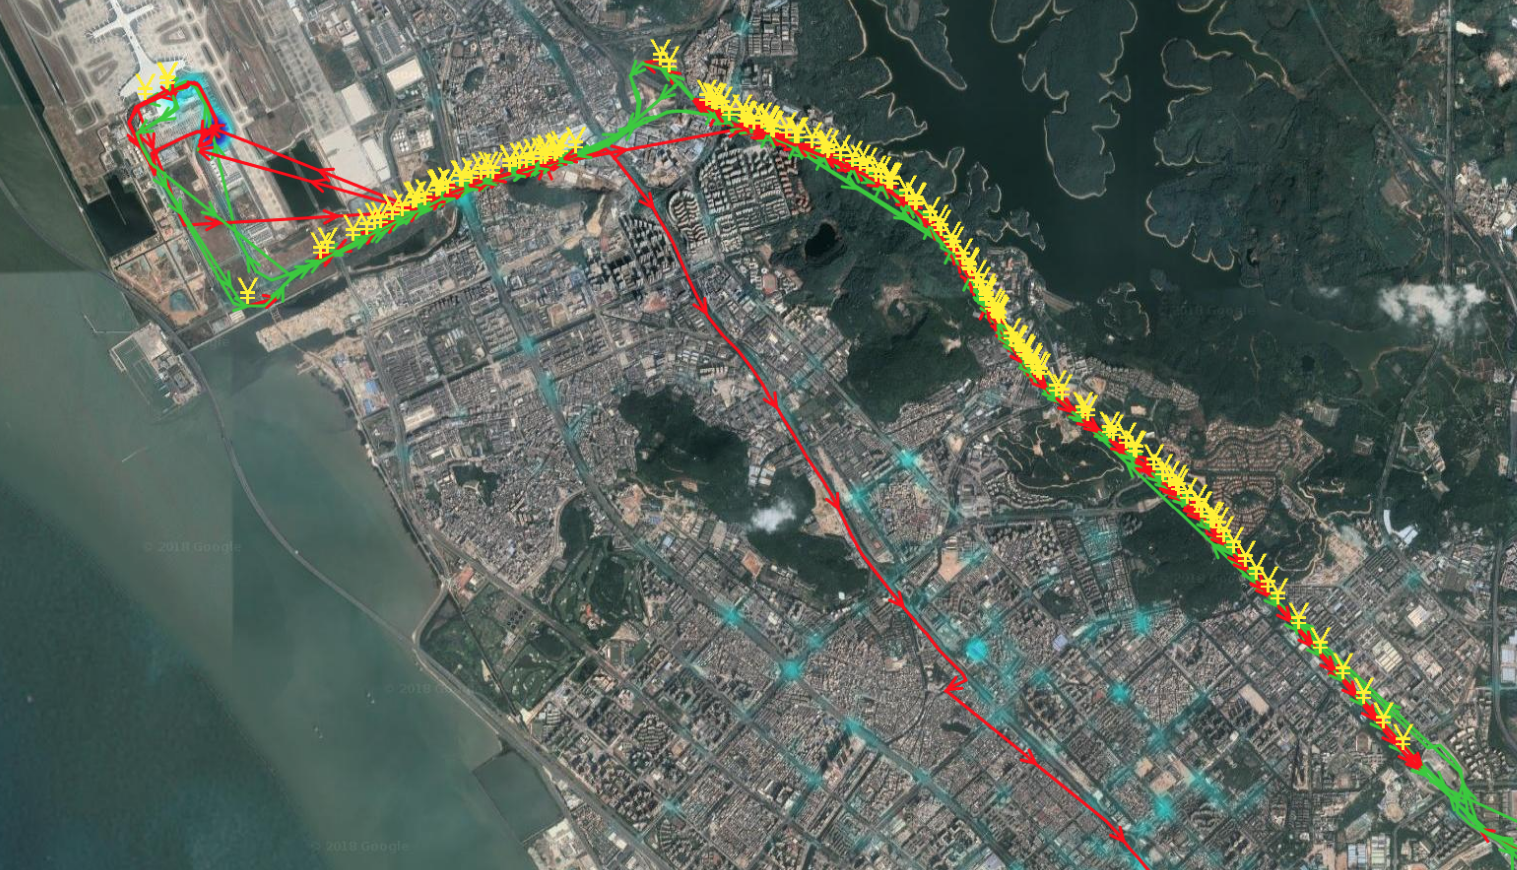
\includegraphics[width=0.5\textwidth]{img/passenger_status.png}
\caption{Passenger status changes every 30 seconds (trajectory with id \textit{27,224})}
\label{fig:passenger_status}
\end{figure}


\subsubsection{Jumps}
GPS data tends to be imprecise by nature. This results in inaccuracies as well as \quotes{jumps}. We define points that are most likely not real based on the driven speed as a jump. In order to get a better understanding of that, we depicted an example in figure \ref{fig:jump}. The green line shows an example route as it also appears in the dataset. The numbers next to the line represent the driven speed in $\frac{km}{h}$ between two points $P_i$ and $P_{i+1}$. Point $P_4$ catches the eye of the observer. The speed of more than $200\frac{km}{h}$ within the city of Shenzhen might not be even possible. To avoid such cases, we developed a Python script, that analyzes the speed between two points. If it is higher than $150\frac{km}{h}$ we take the next point into account. In our example, we calculate the speed between $P_3$ and $P_5$. Is it less than $150\frac{km}{h}$ we delete the point in between (here $P_4$). Otherwise, there is a defect that is not trivially solvable.

\begin{figure}[ht]
\centering
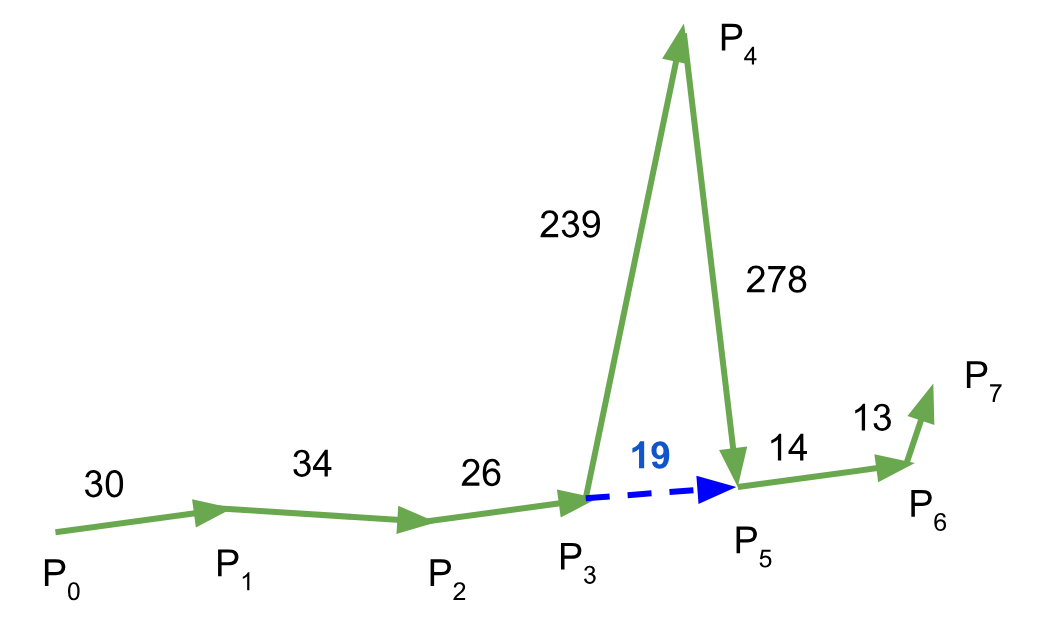
\includegraphics[width=0.5\textwidth]{img/jumps.png}
\caption{Example route containing a jump at $P_4$}
\label{fig:jump}
\end{figure}

In some cases the amount of jumps is enormously high. In such cases, we delete the whole trajectory. More specifically, this means: Every trajectory having more than 200 jumps or having more than 100 jumps that cannot be fixed are removed. One extreme example for this can be seen in figure \ref{fig:more_jumps}.

\begin{figure}[ht]
\centering
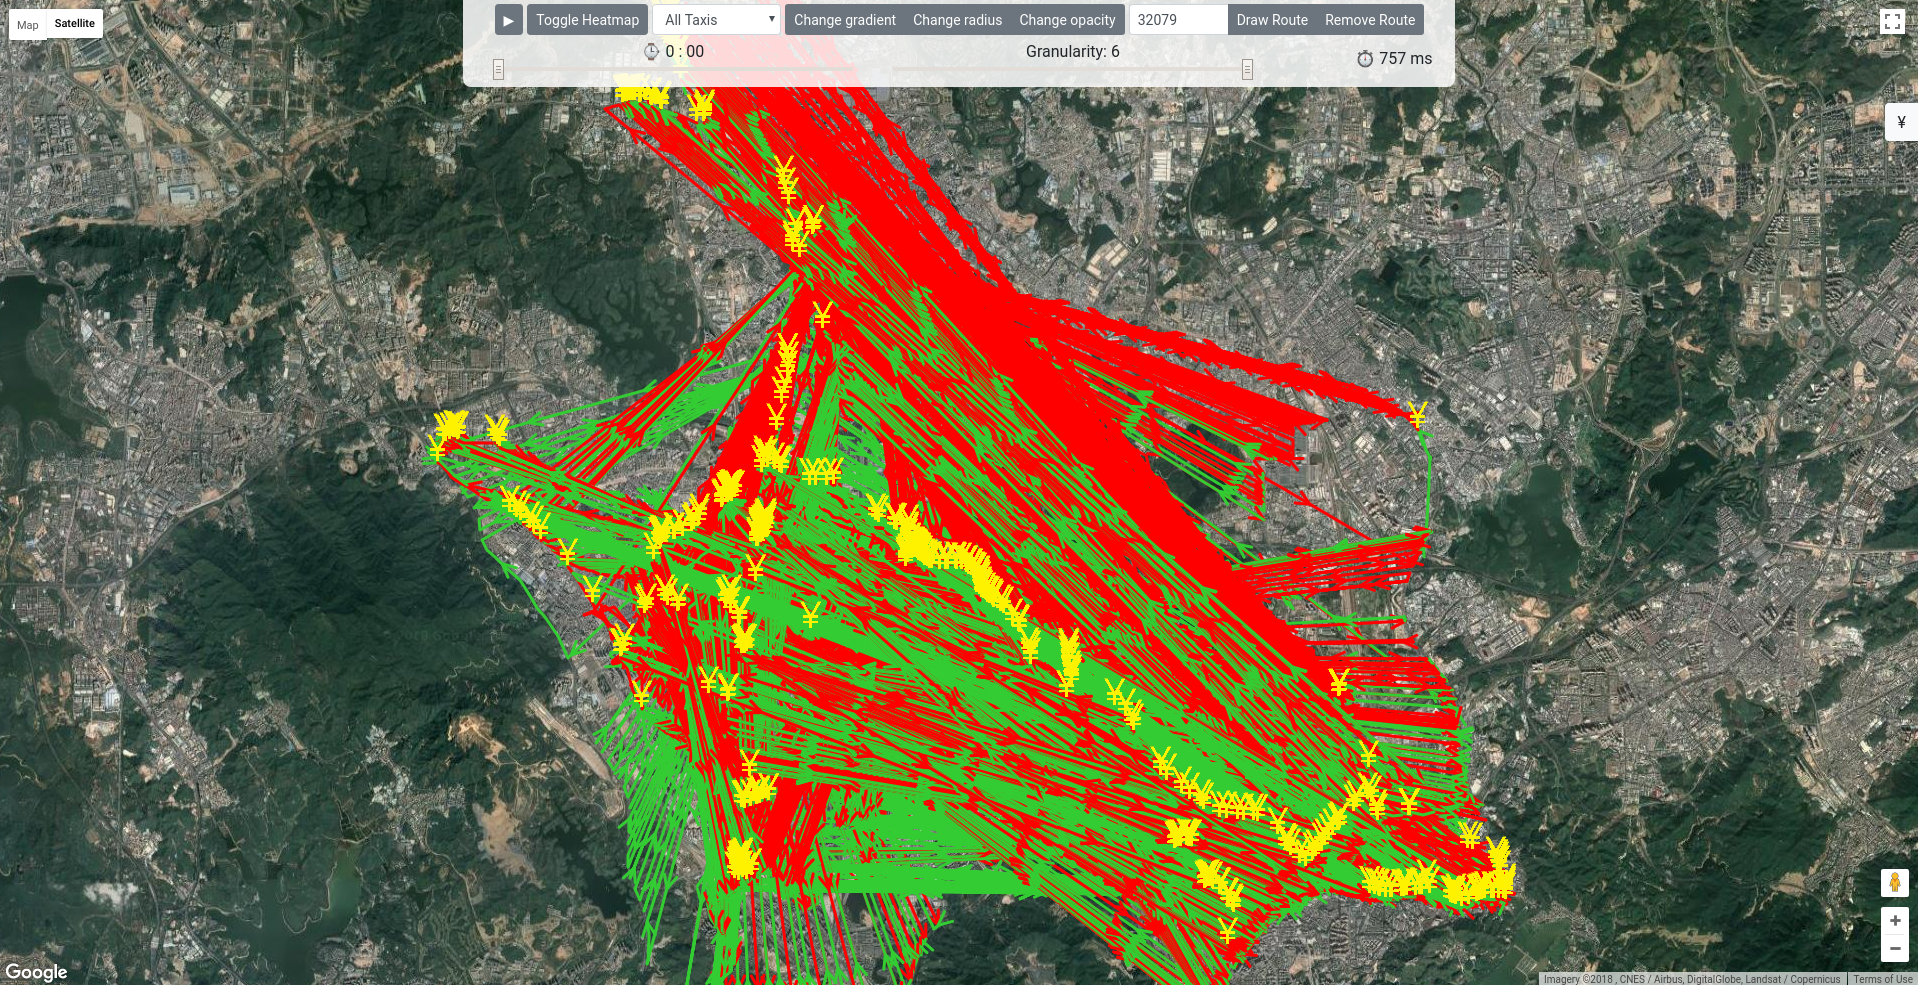
\includegraphics[width=0.5\textwidth]{img/more_jumps.png}
\caption{Trajectory \textit{32,079} having more than 2,000 jumps}
\label{fig:more_jumps}
\end{figure}

\subsubsection{Summary: Data cleansing}
All in all we removed more than eight Million records ($\approx 18\%$) and more than 4,134 trajectories ($28\%$) due to our data cleansing rules. Most of the criteria are chosen generously to avoid deleting false positives. Additionally, there might be other aspects to improve data quality. Since this was not the focus of our work, we decided not to go further into detail.

The following graphics depict the amount of records deleted (see figure \ref{fig:records_deleted}) and the amount of completely removed trajectories (see figure \ref{fig:trajectories_deleted}). The quantities are not disjoint amongst the data cleansing steps. In other words, a record or trajectory can occur in multiple sets. Otherwise, the numbers would depend on the order the data cleansing steps were made.

\begin{figure}[ht]
\centering
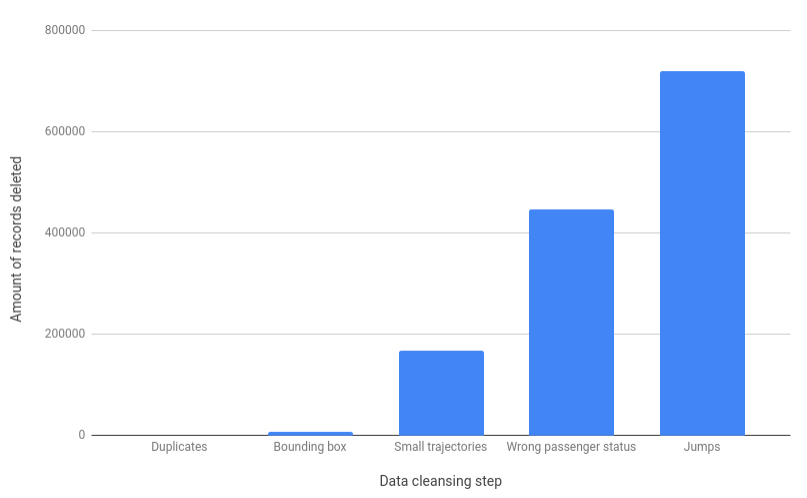
\includegraphics[width=0.5\textwidth]{img/records_deleted.png}
\caption{Amount of records deleted per data cleansing step}
\label{fig:records_deleted}
\end{figure}


\begin{figure}[ht]
\centering
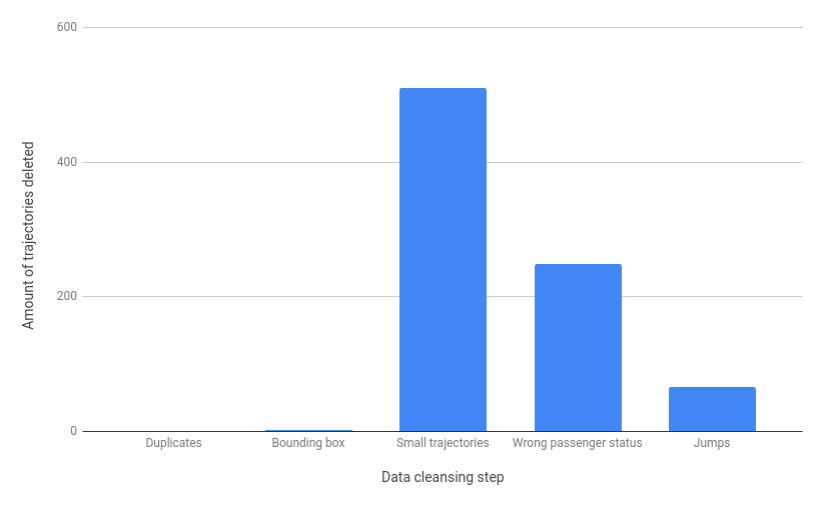
\includegraphics[width=0.5\textwidth]{img/trajectories_deleted.png}
\caption{Amount of trajectories deleted per data cleansing step}
\label{fig:trajectories_deleted}
\end{figure}

\section{Application Prototype}

The main purpose of our application prototype is to display good performing taxis on a map. Thereby, the user can analyze how taxis get new passengers quickly. An additional task is to visualize the state at a certain time of the day. For that, we created some heatmaps (see section \ref{sec:heatmaps}).

\subsection{Taxi Profit Calculation}

The profit can be estimated with the help of the distances and the tours' start and end times. We checked the taxi fares in Shenzhen on the website Numbeo which is a database about taxi fares worldwide\footnote{\href{https://www.numbeo.com/taxi-fare/country_result.jsp?country=China}{https://www.numbeo.com/taxi-fare}}. The website states that the start of a taxi tour costs 11.00 Chinese Yuan. Then it costs 2.40 Yuan per kilometer. We have the GPS coordinates and know where a tour starts and ends. Because of that, we can calculate the driven distance and get an accurate kilometer price.

Waiting time is a component of the tour's price as well. Numbeo says that it is 48 Yuan per hour. We defined for our application that 10 percent of the total time of a tour is waiting time. That is obviously not the real waiting cost for each tour, just a guess. Nevertheless, it should suffice for our prototype. A better approach would be to calculate the speed of the taxis to check if it was waiting or driving at the time.

The prices of all tours can be summed up to the profit of a taxi over the whole day. At this point we have a profit estimation for each taxi.

\subsection{Explore Profitable Taxis}

The user can see a ranking of the taxis, which had the most profit during the day. This is shown in figure \ref{fig:ranking}. The list has information about the number of tours. We also calculated the distance of each taxi while passengers were inside. This is displayed in the column \textbf{Distance km}. The list is sorted by the estimated profit which is explained in the previous section. It is displayed as the Chinese currency Yuan. When the user clicks on an entry the route for the taxi is drawn on the map.

\begin{figure}[ht]
\centering
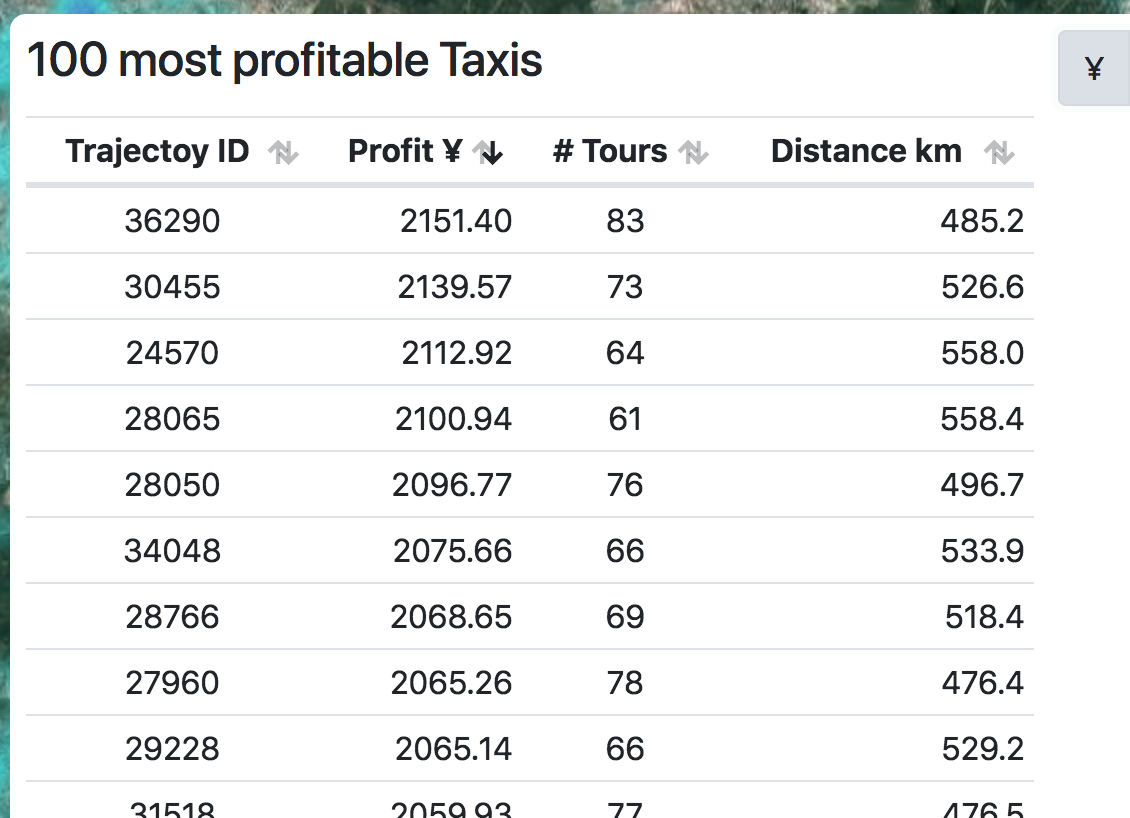
\includegraphics[width=0.5\textwidth]{img/ranking.png}
\caption{Ranking of the most profitable taxis}
\label{fig:ranking}
\end{figure}

The red part of the drawn line indicates the taxi was driven without a passenger. The line is green if it had a passenger. Arrows indicate the direction. At the end of each tour is a Yuan symbol on which the user can click. The click lets some information about the tour (i.e. start time, end time, distance and the estimated profit) pop up.

Figure \ref{fig:best_taxi} shows the route of the most profitable taxi (ID \textit{36290} in figure \ref{fig:ranking}). You can see that this taxi had the most tours in one area. The taxi had 83 tours during the day. These tours sum up to a distance of 482 kilometers. The red lines are often very short.

\begin{figure}[ht]
\centering
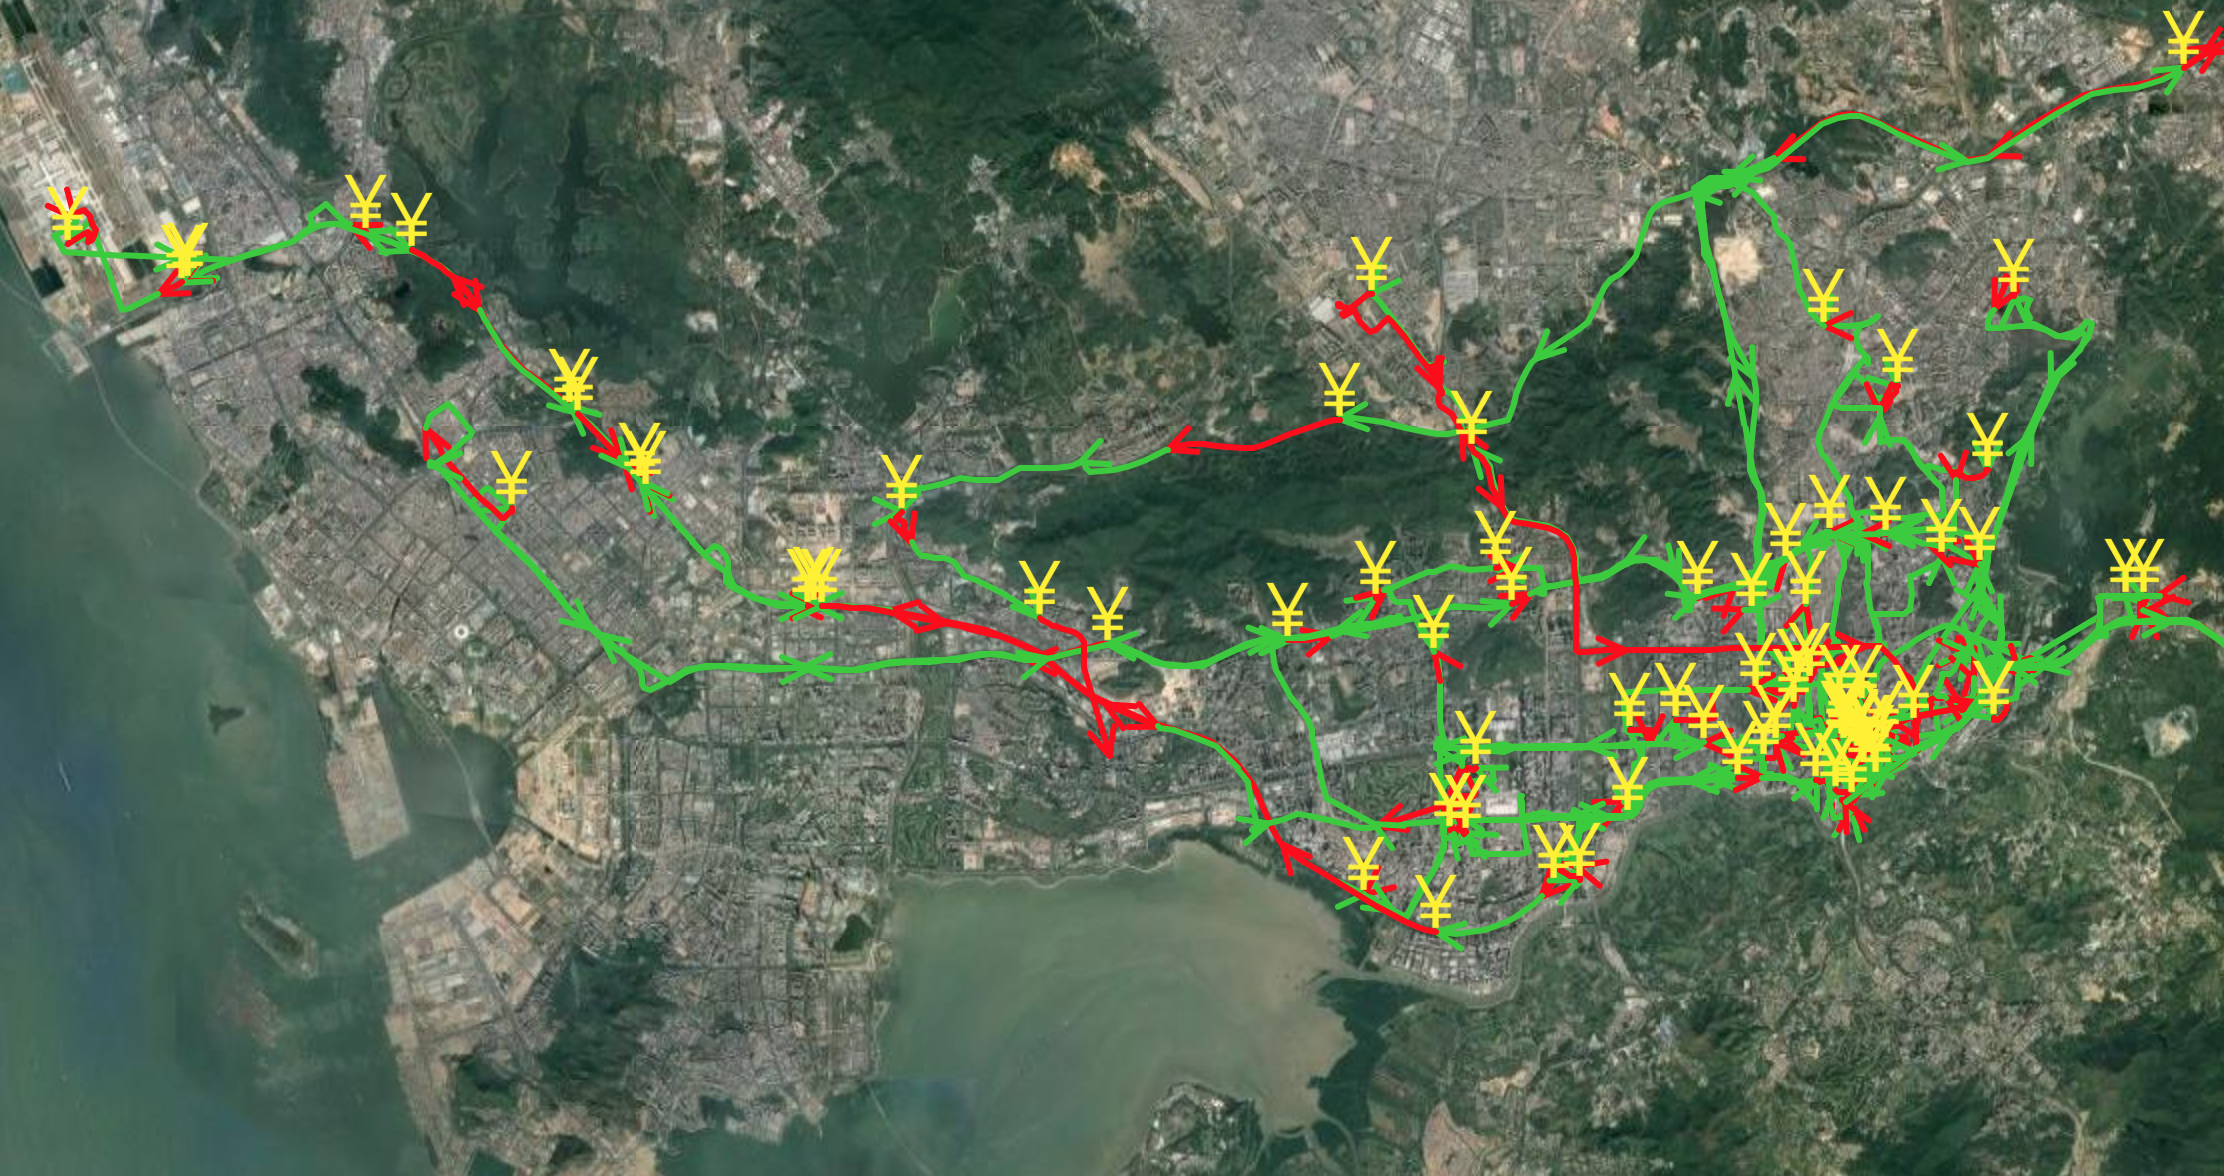
\includegraphics[width=0.5\textwidth]{img/best_taxi.png}
\caption{Entire taxi route}
\label{fig:best_taxi}
\end{figure}

\subsection{Heatmaps}
\label{sec:heatmaps}

The application has a taxi density heatmap. The areas, which have many taxis at the given time, are colored red. Areas with less taxis are colored blue. The user interface has a time slider. When changing the time from 3:00 PM to another time, the map refreshes. In the top left corner is a play button. With the play function, the map continually updates to the next time interval. Thus, the user can observe how the taxi density changes over time.

The heatmap can visualize two other things. One of these is the number of picked up passengers. The other one is the number of dropped passengers. The user interface has a dropdown menu to let the user select which heatmap is displayed.

\subsection{System Architecture}

This section is about our architecture. Figure \ref{fig:architecture} is an FMC (Fundamental Modeling Concepts) diagram. Our architecture can be divided into the three components frontend, backend and database. Since we have a web application, it runs in a browser. We are using the Google Maps API. In our frontend, we are using HTML5 and Javascript.

\begin{figure}[ht]
\centering
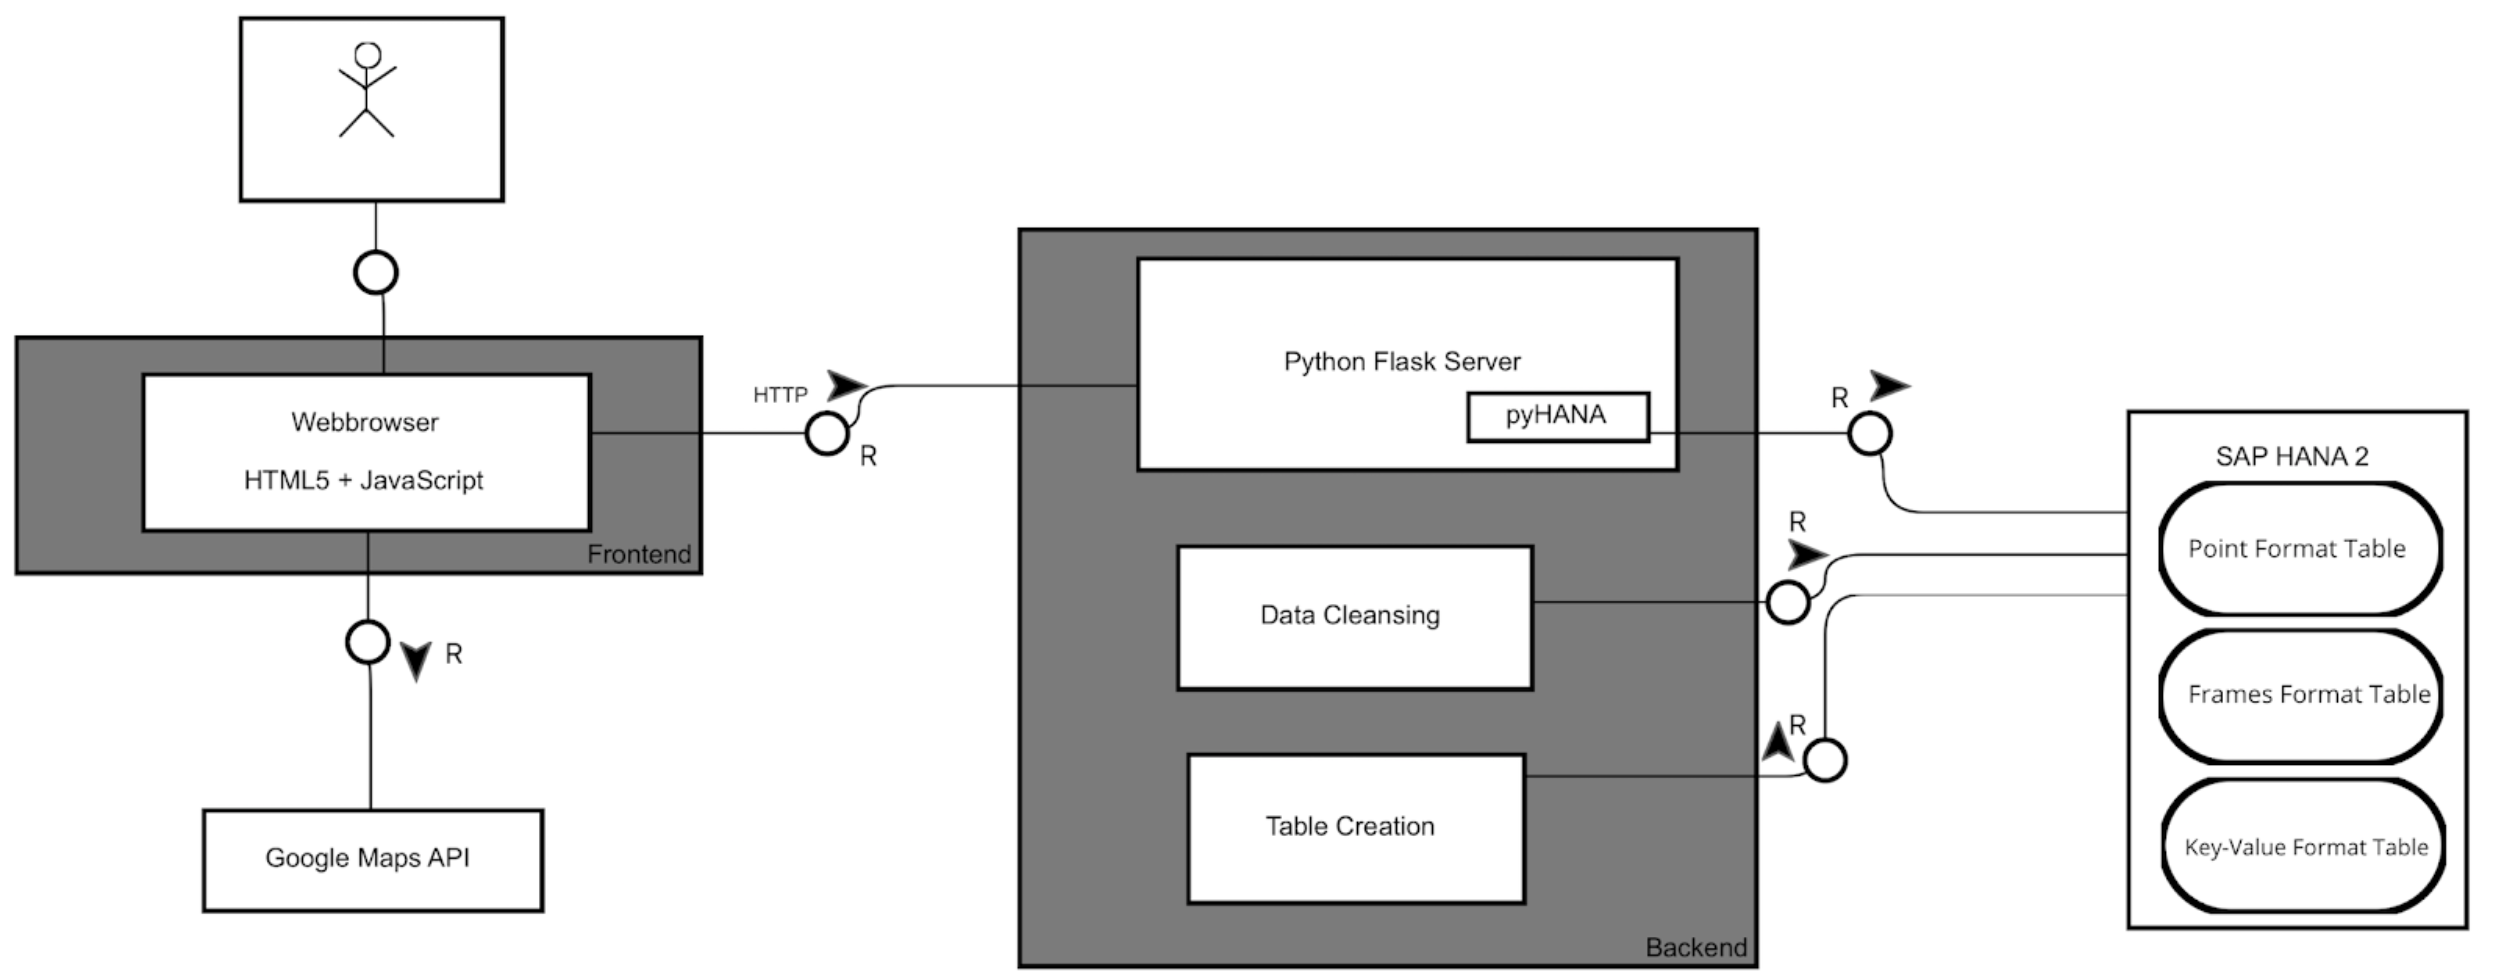
\includegraphics[width=0.5\textwidth]{img/architecture.png}
\caption{System architecture}
\label{fig:architecture}
\end{figure}

The backend essentially has a REST API which is written in Python and uses the Flask framework. It serves the static HTML and Javascript files, as well as redirecting requests to the database. The backend also has a few Python scripts that are used to create tables and perform data cleansing.

The database we are using, is SAP HANA. It stores all the data in different table formats. The table formats are elaborated in section \ref{sec:data_layouts}. The database has some procedures that can be executed to answer non-trivial data requests (e.g. to get the calculated profits).

The communication between the backend and the database in managed via pyHANA\footnote{\href{https://github.com/hpi-epic/pyHANA}{https://github.com/hpi-epic/pyHANA}}. pyHANA is a Python client for SAP HANA.


\section{Data Layouts}
\label{sec:data_layouts}
A crucial factor for SQL query performance is the way the data is stored. Therefore, we tried out three different layouts which we want to present in this section.
\subsection{Sample point format}
The sample point format is similar to the way the data is stored in the CSV-file. Each GPS sample corresponds to one row within the database. Furthermore, each attribute is stored in one column without any manual encoding.

The layout has three major advantages. First, the data can be accessed directly. There is no need for further calculation or modification in order to obtain a specific value. Second, the data stays as it is. Since there is no normalization, we always have the full dataset in hand. Additionally, the amenities of column store can be exploited. SAP HANA supports various internal compression types in order to reduce the amount of memory used. Less data has to be loaded from memory, which leads to a higher throughput and faster query execution times.

The whole table consumes about 498 MB of main memory after applying the data cleansing rules. We prefer the column store over the row store in this case.

\subsection{Frame format}
Another way of storing the information is the frame format. This approach is presented by Wang et al.~\cite{wang} The main idea behind this layout is splitting the sample points into frame groups of a fixed length with a fixed frequency of data points. We decided to use a frame size of 30 seconds and a frame group size of one hour as described in the paper by Wang et al.

To keep the right order of the data points after splitting a trajetory into multiple frame groups a frame group identifier (\textit{FGCID}) has to be introduced (cf. figure \ref{fig:frame_format}). The starting point's GPS location of a frame group is stored in the column \textit{IFX} (latitude) and \textit{IFY} (longitude). In order to save memory the subsequent points are encoded as the deltas of the coordinates. The columns are named \textit{PF0X, PF0Y, PF1X, PF1Y, ..., PF119X, PF119Y}. Hence, the frame format table consists of 244 columns.

\begin{figure}[ht]
\centering
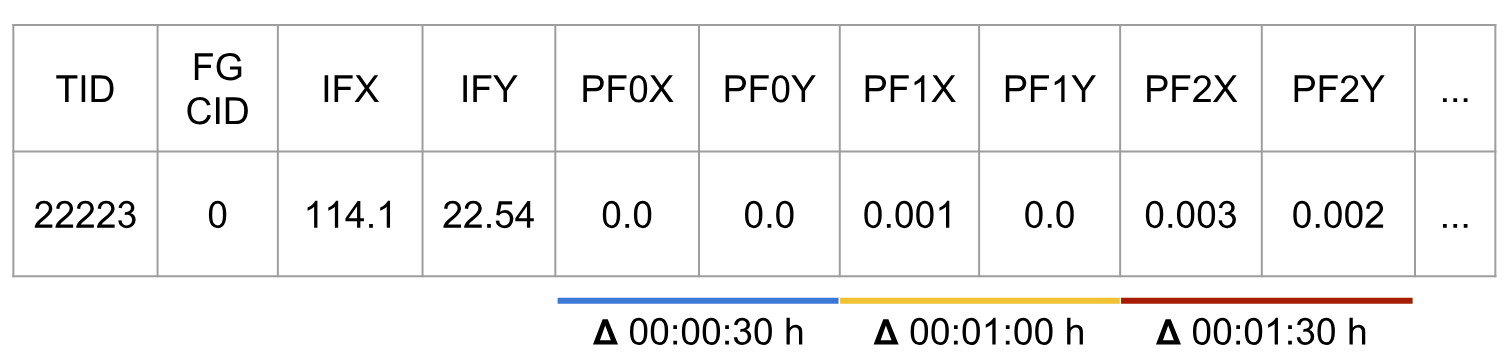
\includegraphics[width=0.48\textwidth]{img/frame_format.png}
\caption{Information stored in frame format}
\label{fig:frame_format}
\end{figure}

This approach avoids using timestamps, which is a major advantage in terms of memory consumption. Also querying a time series is supposed to be faster compared to the frame format. However, the different positions within the frames have to be calculated, which can be a tedious thing. Due to the use of frames the data is normalized by time on the one hand. On the other hand, there is a loss of information. Furthermore, there could be the possibility of missing points. In this case, Wang et al.~\cite{wang} calculate those points via computing the SED distance. We refrain from that. The overall frame format table with a framegroup size of one hour and a frame size of 30 seconds consumes circa 441 MB of main memory, when stored in column layout. In total, there are more than 2 million rows.

\subsection{Key-Value format}

A third storage layout we evaluated is the key-value format. Therefore, we decided to encode a whole trajectory as an array of arrays containing longitude, latitude and the corresponding timestamp. Since an array cannot be stored in the SAP HANA database directly, we take its string representation and filed it in a column of data type \textit{NCLOB}. An example can be found in code listing \ref{lst:json}. We do not normalize by time. Hence, there is no loss in terms of GPS data. Besides this information, there are the trajectory identifier, start and end time and the mininum bounding rectangle present in the table. In total, there are 10,594 (equivalent to the amount of trajectories after data cleansing) consuming about 650 MB of main memory in column store.

\lstset{language=json}
\begin{minipage}{0.45\textwidth}
\begin{lstlisting}[frame=single, firstnumber=1, caption=Key-Value format example entry,label=lst:json]
"[
    [
        "0001-01-01 00:00:03",
        22.512432,
        113.913933
    ],
    [
        "0001-01-01 00:00:58",
        22.5163,
        113.917068
    ],
    ...
]"
\end{lstlisting}
\end{minipage}


\subsection{Optimizations}

\subsubsection{Sample point format}

Since the data neither changes nor grows anymore, we decided to store the information in sorted order. As sorting key we utilized the trajectory identifier and the timestamp. In order to speed up window queries we materialized a unique identifier, which is the row ID. This ID simplifies the creation of a primary key. Otherwise, a primary key would have to include multiple columns, most likely all of them. The HANA database automatically creates an index on this column. Furthermore, we realized that timestamp operations perform relatively bad. In order to avoid timestamps we calculate the amount of seconds lasted since midnight and store those as an integer in the database.

\subsubsection{Frame format}
Wang et al.~\cite{wang} have chosen a frame size of 30 seconds. In our opinion, this interval is relatively large. As presented in section \ref{sec:ds} the median frequency of data points is 15 seconds. Therefore, we adopted the frame size. By changing this value, the frame group size increases as well. This would lead to having 484 columns in the frame format table. Querying data becomes an error-prone task. Thus, we decreased the frame group size to ten minutes.

Additionally, we added the information of speed and occupancy per frame. Those fields are important for our application.

\section{Benchmark results}
Our application executes several SQL statements. In order to improve their speed, we had to decide for one data storage layout per query during application development. Therefore, we created some benchmarks, which we want to present in this section. Moreover, we created benchmarks for use cases, that are not relevant for our software.

\subsection{Application specific benchmarks}
In this section we present the benchmark results of the queries directly related to our application.

\subsubsection{Get whole trajectory}
In various situations we need to have a whole trajectory in hand. Therefore, we wrote SQL queries for each storage layout. The query execution times are shown in graphic \ref{fig:bench_whole_trajectory}. In order to create the statistics we ran the queries 100 times. The time is measured within our Python server and encompasses the whole recreation. Network latency between the server and the database has not been measured. Hence, it is not part of the benchmark.

The slowest query execution time has the sample point format. Anyway, the data retrieved from the database does not need to be recreated in the Python backend. It can be used as it is.

Recreating a trajectory in the frame format is faster in terms of retrieving the data from the database. However, in order to calculate the correct GPS coordinates there is a computation overhead. We have done this in the Python backend. An attempt of recreating the data via an SQL procedure using dynamic SQL failed due to extraordinary execution times. This takes 89.3 seconds, which is a performance decrease by factor 4000. An explanation for the high number could be, that dynamic SQL cannot be optimized well by the DBMS and runs in a single threaded style. An analysis of the query was not possible in this case, because the name server keeps crashing if we do so. The frame layout having a frame size of 15 seconds almost takes double the time as the frame size of 30 seconds. The reason for that, is the double amount of data.

The fastest approach of trajectory recreation is the key-value format with an execution time of 9.5 microseconds. Querying the database becomes the fastest part, because only a single field is required. A huge amount of time is consumed by parsing the JSON string and creating a JSON object. Parsing the string within an SQL command does not represent an option for us, since this way is toos error-prone.

\begin{figure}[ht]
\centering
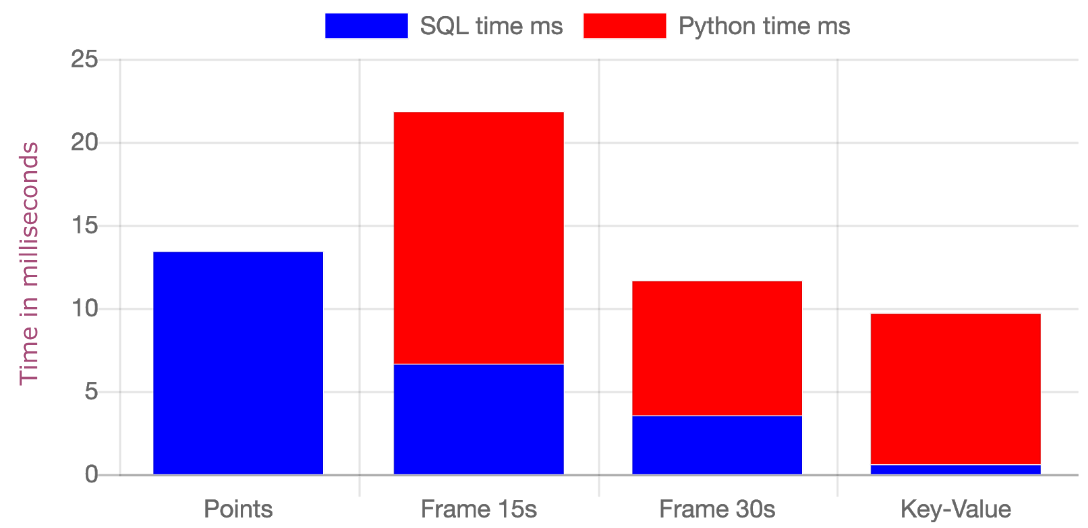
\includegraphics[width=0.48\textwidth]{img/bench_whole_trajectory.png}
\caption{Time required for retrieving one trajectory}
\label{fig:bench_whole_trajectory}
\end{figure}


\subsubsection{Calculate distances}
A key functionality of our software is the calculation of the profit per taxi. Therefore, we take three different factors into account:
\begin{enumerate}
    \item Taxi start: As soon as a passenger enters a taxi, he or she has to pay 11 Yuan.
    \item Waiting time: There are several reasons why a vehicle has to wait (e.g. for the passenger). We assume, that this time is approxiamtely 10 percent of the ride. An hour of waiting time costs 48 Yuan.
    \item Distance driven: The price of a ride depends on the distance. A typical value is 2.40 Yuan in the city of Shenzhen.
\end{enumerate}
% Die Werte haben sich schon geändert ;)
The prices used for calculation are taken from a website.\footnote{\href{https://www.numbeo.com/taxi-fare/country\_result.jsp?country=China}{https://www.numbeo.com/taxi-fare/country\_result.jsp?country=China}} The values might have changed until now. However, prices will not change in a way, that our calculations become fundamentally wrong.

The calculation of aspect one and two is trivial since these are only simple additions or multiplications. Determining the distance is a more complex part, that we want to describe in detail now.

To calculate the distance, we want to do it completely in the database. When querying a full trajectory we have to use the sample point format, since any other layout depends on the Python backend.

The simplest way to get the distance of a ride is the usage of spatial points (\textit{ST\_POINTS}). This is a data type implemented in SAP HANA, that can be created out of a longitude and a latitude value. Furthermore, there is a function to compute the distance between those points. A single ride starts, when a passenger enters a taxi (occupancy changes from zero to one) and ends, when the passenger leaves (occupancy changes from one to zero). We sum up the lengths between all points and all values for a whole trajectory.

We performed a first run on the original unoptimized table. This takes more than eight minutes. A query execution of such a high duration is far away from real time computing. Luckily, we have an improved table. However, the query execution time still takes 198 seconds, which is way to high. When looking into the query plan, we immediately see that the conversion of longitude and latitude to \textit{ST\_POINTS} takes a tremendous amount of time (roughly 133 seconds). We then materialized the \textit{ST\_POINTS}. The query now runs within 65 seconds. Compared to the eight minutes of the initial approach this result sounds great. Anyway, this duration is still too high to calculate the distances on demand.

Once again, a look into the query plan clarifies the problem. Almost 70 percent of the time is spent in determining the displacement between the points. When using \textit{ST\_POINTS} the use of \textit{st\_distance} cannot be avoided. Another alternative we considered is the implementation of an own method to compute the distances. The haversine formula seems to be well suited for our purpose. It determines the displacement of two points on a spherical object. The formula is defined as follows:

\begin{equation} a = sin^2(\frac{\Delta_{lat}}{2}) + cos(lat_1) \cdot cos(lat_2) \cdot sin^2(\frac{\Delta_{lon}}{2}) \end{equation}
\begin{equation} c = 2 \cdot atan2(\sqrt{a}, \sqrt{1 - a}) \end{equation}
\begin{equation} d = R \cdot c \end{equation}

where $lat$ is the latitude, $lon$ the longitude and $R$ the Earth's radius, which is 6,367,000 meters. Since the radius depends on the location on the Earth, we assume a slight deviation. In fact, the standard deviation is 95 meters respectively 0.04 percent compared to the results of \textit{st\_distance}. Indeed, the query execution time reduces to 7.6 seconds. This is a speed up of factor 8.5 . With this solution a calculation on demand becomes possible.

\subsubsection{Get points from timeframe}
For our heatmap it is necessary to get all taxis within a specific time frame. With every returned GPS point the heatmap also gets a weight which indicates the number of taxis there. It is also possible to change the granularity of those GPS points. We did not implement this task for the key-value format, because the overhead of parsing the large string as JSON object before any further operations can be performed is too much.

For the point format all entries are simply filtered by their timestamp to be within the given period and, depending on the desired granularity, rounded to a different amount of decimals. Afterwards the results are grouped by latitude and longitude to get the weight. This takes about 19 milliseconds.

As the frame format is geared to such time frames it should be much faster to get all points within a frame. Figure \ref{fig:bench_whole_trajectory} shows that with 14 milliseconds it is faster than the point format, but only by a small amount. The reason for that is the delta encoding for all but the first coordinate within a frame. So, for each entry found the coordinate needs to be calculated. After this is done, rounding the coordinates according to the granulatrity and grouping to get a weight is the same as for the point format.
\begin{figure}[ht]
  \centering
  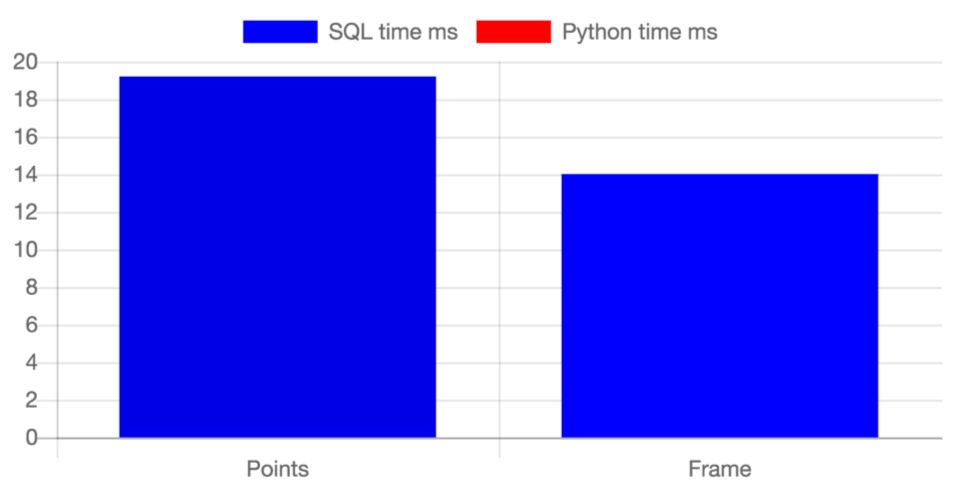
\includegraphics[width=0.48\textwidth]{img/bench_single_frame.png}
  \caption{Time in microseconds required for retrieving one single time frame}
  \label{fig:bench_whole_trajectory}
\end{figure}

\subsection{Application independent benchmarks}
We tried to improve the SQL statement performance on many ways. Sometimes our anticipated improvements did not occur. Nevertheless, we want to present those failed optimizations. We also ran queries not related to our application, because we want to have a broader comparison between the different layouts.

\subsubsection{Storing floats as two integers}
Floating point operations tend to be slower than integer operations. We split up each float column for latitude and longitude into two integer columns with the intention to speed up calculations. For the test we filtered all entries to be within a given bounding rectangle. In fact, this aproach more than doubled the processing time of the query for multiple integer columns compared to the single float ones as depicted in Figure \ref{fig:bench_coordinates_as_int}.
\begin{figure}[ht]
  \centering
  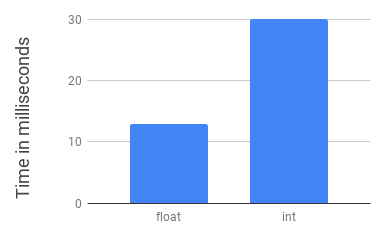
\includegraphics[width=0.48\textwidth]{img/bench_coordinates_as_int.png}
  \caption{Time in ms filtering by coordinates}
  \label{fig:bench_coordinates_as_int}
\end{figure}

\subsubsection{Storing time in multiple columns}
One successful optimization was to store time as seconds instead of timestamps. But when filtering by time often the hours, minutes or seconds part of a time data point is important. With that in mind, we stored the timestamps in three colums for the hour, minutes and seconds part with the purpose of better access and faster filtering. However, as illustrated in Figure \ref{fig:bench_time_as_multiple_ints} our measurements showed that filtering by time became three times slower than with just using seconds.
\begin{figure}[ht]
  \centering
  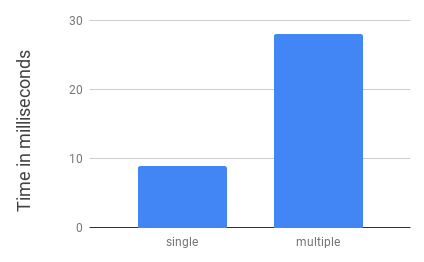
\includegraphics[width=0.48\textwidth]{img/bench_time_as_multiple_ints.png}
  \caption{Time in ms required for filtering by time}
  \label{fig:bench_time_as_multiple_ints}
\end{figure}

\subsubsection{Get taxis in time and range boundary}
We wanted to find out how these last two optimizations perform on a more complex query of a realistic scenario: retrieving all taxis within a defined time period and geografic bounding rectangle. We implemented this rather complex statement as prcedure for easy usage. Figure \ref{fig:bench_time_range_boundary} shows that the execution time of the multiple columns approach dramatically exceeds the single column approach with increasing number of results.
\begin{figure}[ht]
  \centering
  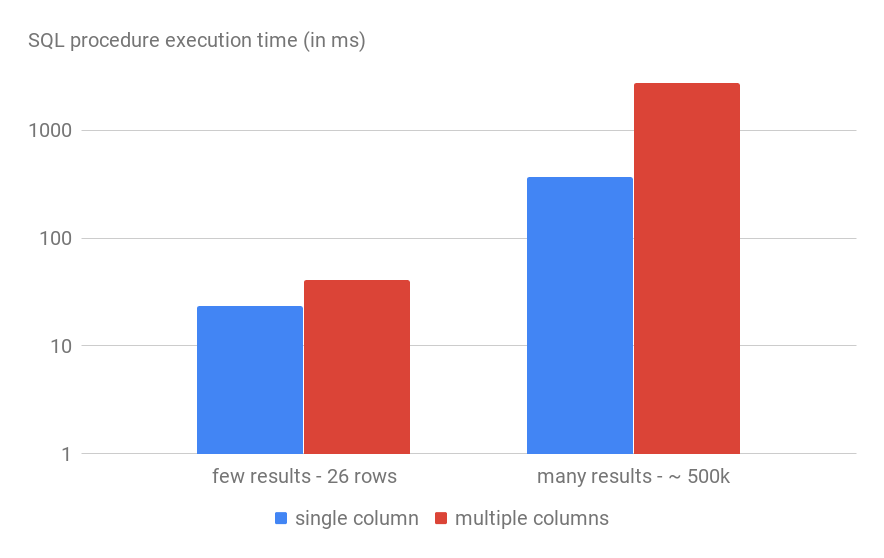
\includegraphics[width=0.48\textwidth]{img/bench_time_range_boundary.png}
  \caption{Time in ms required for filtering by coordinates and time}
  \label{fig:bench_time_range_boundary}
\end{figure}

\section{Conclusion}
We managed to optimize the performance of many of our queries for each data layout. Nevertheless, none of the formats excels in all cases.

The frame format gears to the time aspect of trajectory data. So it suits best when queries are about the continuous points within a time frame. For our example use case, we are rather interested in specific points in time or aggregated information about a timespan. Therefore, before the data has the desired format to work with, some additional steps always have to be calculated every time. This extra work leads to loosing advantage in performance comapred to the point format.

For location specific queries like those in our sample application, the point format suits well, because most times no furthermore calculations are necessary to query the data properly.

The key-value format does not at all fit a column-based database, because for every query almost the entire table has to be loaded and parsed in the application before any selection is possible. Also, the maximum bounding rectangle and start as well as end time in separate columns were not helpful in our specific case, as every entry of our dataset covered a very similar time and spacial span. This format should be implemented in a document store database for a appropriate evaluation.

In the end it strongly depends on a concrete use case which data layout to use and how to optimize it. Furthermore, for each use case, the tradeoff between memory usage and performance has to be found.

We experienced that SAP HANA as our columnar in-memory database is very fast in calculations and aggregations. It also has good compression rates. Especially for our use case, data modification and operations on timestamps were necessary, which we found out to be rather slow. Nevertheless, this can partly be overcome by some of our optimizations.

% \bibliographystyle{ACM-Reference-Format}
\bibliographystyle{plain}
\bibliography{references}

\end{document}
